\documentclass[11pt,letterpaper]{article}

% ---------- page and type ----------
\usepackage[top=1.05in,bottom=1.05in,left=1.2in,right=1.2in,headsep=0.3in]{geometry}
\usepackage[T1]{fontenc}
\usepackage[utf8]{inputenc}
\usepackage{XCharter}
\renewcommand{\ttdefault}{lmtt}
\usepackage[final]{microtype}
\linespread{1.12}
\setlength{\parindent}{0pt}
\setlength{\parskip}{0.62em}
\raggedbottom
\renewcommand{\topfraction}{0.9}\renewcommand{\bottomfraction}{0.8}\renewcommand{\textfraction}{0.08}\renewcommand{\floatpagefraction}{0.8}
\setlength{\textfloatsep}{1.4em}\setlength{\intextsep}{1.2em}

\usepackage{xcolor}
\definecolor{ink}{HTML}{1A1A1A}
\definecolor{muted}{HTML}{5F5E5A}
\definecolor{accent}{HTML}{1C5CAB}
\definecolor{rule}{HTML}{D8D6D0}
\definecolor{panel}{HTML}{F6F5F1}
\definecolor{factor}{HTML}{2A78D6}
\definecolor{pca}{HTML}{EB6834}
\color{ink}

\usepackage{graphicx,booktabs,array,tabularx,float,enumitem,amsmath}
\usepackage[font={small,color=muted},labelfont={bf,color=ink},labelsep=period,skip=6pt]{caption}
\usepackage{titlesec,fancyhdr,listings,tikz}
\usetikzlibrary{arrows.meta,positioning}
\usepackage[most]{tcolorbox}
\usepackage[colorlinks=true,linkcolor=accent,urlcolor=accent,
  pdftitle={Fundamental Factors vs. PCA: Comparing Two Risk Models for Tracking the S\&P 500},pdfauthor={Rayhan Driver}]{hyperref}

\graphicspath{{../figures/}}
\setlist{itemsep=0.25em,topsep=0.3em,leftmargin=1.4em}

% ---------- headings ----------
\titleformat{\section}{\Large\bfseries}{\textcolor{accent}{\thesection}}{0.7em}{}
\titlespacing*{\section}{0pt}{1.7em}{0.45em}
\titleformat{\subsection}{\normalsize\bfseries}{\textcolor{accent}{\thesubsection}}{0.6em}{}
\titlespacing*{\subsection}{0pt}{1.1em}{0.15em}

% ---------- header and footer ----------
\pagestyle{fancy}\fancyhf{}
\renewcommand{\headrulewidth}{0pt}
\fancyhead[L]{\footnotesize\color{muted}\textsc{Fundamental factors vs.\ PCA}}
\fancyhead[R]{\footnotesize\color{muted}Rayhan Driver}
\fancyfoot[C]{\footnotesize\color{muted}\thepage}
\fancypagestyle{first}{\fancyhf{}\fancyfoot[C]{\footnotesize\color{muted}\thepage}}

% ---------- small helpers ----------
\newcommand{\F}{\textcolor{factor}{\textbf{Factor}}}
\newcommand{\Pc}{\textcolor{pca}{\textbf{PCA}}}
\newtcolorbox{takeaway}{enhanced,breakable,colback=panel,colframe=panel,boxrule=0pt,arc=2pt,
  borderline west={2.2pt}{0pt}{accent},left=11pt,right=11pt,top=7pt,bottom=7pt,
  before skip=0.9em,after skip=0.9em,before upper={\setlength{\parskip}{0.55em}}}
\lstset{language=Python,basicstyle=\ttfamily\footnotesize,columns=fullflexible,keepspaces=true,
  commentstyle=\color{muted},keywordstyle=\color{accent},stringstyle=\color{muted},
  showstringspaces=false,backgroundcolor=\color{panel},frame=single,rulecolor=\color{panel},
  framesep=7pt,xleftmargin=8pt,xrightmargin=8pt,aboveskip=0.9em,belowskip=0.7em
}

\begin{document}
\thispagestyle{first}

% ---------- title block ----------
{\footnotesize\color{accent}\textsc{\MakeLowercase{Research whitepaper}}\hfill
 \color{muted}Summer 2026 internship, Alphathena}

\vspace{0.9em}
{\fontsize{22}{27}\selectfont\bfseries Fundamental Factors vs.\ PCA:\\[1pt] Comparing Two Risk Models for\\[1pt] Tracking the S\&P 500\par}

\vspace{0.7em}
{\large\color{muted} An out-of-sample study for direct indexing, 2018 to 2025\par}

\vspace{1.1em}
{\small \textbf{Rayhan Driver}\quad\textcolor{muted}{with Tommy Bobitz, partner intern}\hfill
 \textcolor{muted}{November 2026}}

\vspace{0.5em}
{\color{rule}\hrule height 0.8pt}
\vspace{1.0em}

% ---------- summary ----------
\begin{takeaway}
\textbf{Summary.} Last summer my partner intern and I built a new risk model for a
direct-indexing platform and tested it against the model the firm already used. Ours named
its risk drivers in advance (value, momentum, size, sector, and so on). The existing one
finds its drivers statistically from price history, using principal component analysis (PCA).

We compared the two on eight years of data the models had never seen, rebuilding both every
month and scoring what happened next. On the main test our model lost, because PCA produced
slightly lower risk on a broad S\&P 500 portfolio and the gap held up under a significance
test. Our model did trade about 25\% less, performed better on small and concentrated
portfolios, and picked more sensible replacement stocks for tax-loss harvesting. A simple
blend of the two models matched PCA on tracking.

The most useful outcome was a clear picture of where each model performs better, backed by
checks showing that the comparison itself was fair.
\end{takeaway}

\begin{table}[H]
\centering\small
\begin{tabular}{@{}lrrl@{}}
\toprule
\textbf{Measure} & \F & \Pc & \textbf{Better} \\
\midrule
Volatility of the minimum-variance portfolio & 17.93\% & 17.07\% & PCA, significant \\
Tracking error against the S\&P 500 & 1.80\% & 1.74\% & PCA, significant but small \\
Turnover of the minimum-variance portfolio & 0.208 & 0.278 & Factor, about 25\% less \\
Sharpe ratio of the minimum-variance portfolio & 0.567 & 0.520 & Factor, not tested \\
\bottomrule
\end{tabular}
\caption{Results for both models on the full S\&P 500 universe, measured out of sample over
96 monthly rebalances from 2018 to 2025. Lower values are better for volatility, tracking
error, and turnover, while a higher Sharpe ratio is better.}
\label{tab:scorecard}
\end{table}

\vfill
{\footnotesize\color{muted} This paper is my own account of research done during an
internship at Alphathena, written for a general technical reader. It is not an Alphathena
publication, it does not describe the firm's production systems in detail, and nothing in
it is investment advice. The portfolios are research constructions, not client results.\par}
\newpage

% =====================================================================
\section{Background}

Direct indexing is an alternative to buying an index fund. An index fund gives an investor
one security that holds the whole index, while direct indexing gives the investor the
underlying stocks themselves. Owning the stocks
directly means the portfolio can be customized, and it means individual positions that have
fallen can be sold to realize a tax loss while the portfolio as a whole keeps following the
index. That second practice is called tax-loss harvesting. Alphathena builds software that
lets financial advisors run portfolios this way.

A direct-indexing portfolio usually holds far fewer stocks than its index, so something has
to decide which stocks to hold, and in what amounts, to follow the index closely. That
decision is made by an optimizer, and the optimizer's main input is a \emph{covariance
matrix}, which estimates how every stock moves with every other stock. With a good estimate,
a portfolio of 150 stocks can behave much like an index of 500, and with a poor one the
portfolio gradually drifts away from the index.

Before this project, the firm built its covariance matrix from prices alone using PCA, which
looks at roughly two years of returns and extracts the patterns of co-movement that explain
the most variance. The approach works well, but the patterns it finds have no names, so
nobody can look at one and say that it represents ``value'' or ``energy.''

A fundamental factor model takes the opposite approach. It decides in advance what the
shared drivers of risk are and then measures each stock's exposure to them, giving up some
statistical fit in exchange for a model people can read. We wanted to know whether it could
also forecast risk as well as PCA. Our claim, written down before we ran anything, was that
a factor model would \emph{control risk at least as well as PCA while trading less}. The
results supported the second half of that claim but not the first.

% =====================================================================
\section{Building the fundamental factor model}

Both models describe risk the same way: a small number of shared drivers that move many
stocks at once, plus each stock's own independent risk. The factor model writes this as
\[
\Sigma \;=\; X F X^{\top} + D ,
\]
where $X$ holds each stock's exposure to each factor, $F$ describes how the factors move
together, and $D$ holds each stock's own leftover variance. We used 20 factors: nine style
scores (beta, growth, liquidity, momentum, quality, size, value, volatility, yield) and the
eleven GICS sectors.

\begin{figure}[H]
\centering
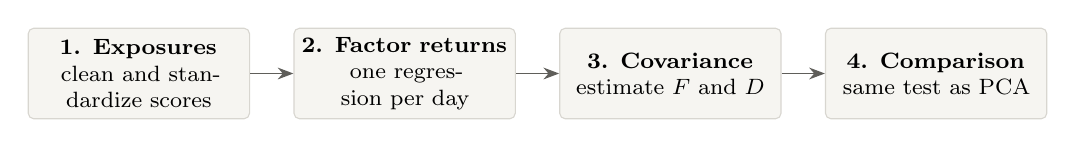
\begin{tikzpicture}[node distance=5.5mm,
  box/.style={draw=rule,fill=panel,rounded corners=2pt,minimum height=11.5mm,text width=26mm,
              align=center,font=\footnotesize,inner sep=3pt},
  arr/.style={-{Stealth[length=2mm]},color=muted,line width=0.6pt}]
\node[box] (a) {\textbf{1. Exposures}\\ clean and standardize scores};
\node[box,right=of a] (b) {\textbf{2. Factor returns}\\ one regression per day};
\node[box,right=of b] (c) {\textbf{3. Covariance}\\ estimate $F$ and $D$};
\node[box,right=of c] (d) {\textbf{4. Comparison}\\ same test as PCA};
\draw[arr] (a)--(b); \draw[arr] (b)--(c); \draw[arr] (c)--(d);
\end{tikzpicture}
\caption{The four stages of building the factor model and preparing it for a direct
comparison with PCA.}
\end{figure}

\subsection{Stock exposures}

For about 6,600 US stocks, we took each company's nine style scores and its sector,
standardized the scores across stocks on each date, and limited the influence of outliers.

\subsection{Daily factor returns}

Each day, we regressed that day's stock returns on that day's exposures, giving larger
companies more weight. The coefficients represent what each factor ``earned'' that day, and
the residuals represent each stock's own move. The core of the regression takes only a few
lines of code:

\begin{lstlisting}
def cross_sectional_regression(y, Xc, weights=None):
    """One day's regression of stock returns on factor exposures.

    y       : Series of stock returns for the day, indexed by ticker
    Xc      : DataFrame of standardized exposures (same tickers, one column per factor)
    weights : per-stock weights (we used the square root of market cap)
    """
    if weights is None:
        weights = pd.Series(1.0, index=y.index)
    rw = np.sqrt(weights)                    # weighted least squares as OLS on scaled rows
    Xw, yw = Xc.mul(rw, axis=0), y * rw
    coef, *_ = np.linalg.lstsq(Xw.values, yw.values, rcond=None)
    f = pd.Series(coef, index=Xc.columns)    # what each factor earned today
    eps = y - Xc @ f                         # what is left over, per stock
    return f, eps
\end{lstlisting}

\subsection{Covariance estimates}

From the history of factor returns we estimated $F$, and from the history of residuals we
estimated $D$, in both cases weighting recent days more heavily. The weighting speeds were
conventional values fixed in advance, and we deliberately did not tune them, since tuning
them on the test data would have given the factor model an unfair advantage.

\subsection{Matching the PCA model's output}

We wrote the new model to produce output in the same form as the PCA model, so that the two
could be run through an identical test with nothing else changed.

% =====================================================================
\section{How we tested the two models}

\subsection{A rolling test with no look-ahead}

On the first trading day of each month from
2018 through 2025, we built both covariance matrices using only data available on that day,
formed portfolios from each, and then recorded how those portfolios actually behaved over
the following month. That gave 96 rebalances and 2,010 trading days of results. The rule
against using future data was enforced where the data is read from disk, so a later-dated
row could not reach an earlier estimate by accident. The universe was the S\&P 500 stocks
for which we had complete data at each date: about 450 names on average, covering roughly
93\% of the index by weight.

\subsection{The portfolios used to score each model}

We formed two portfolios from each model's covariance matrix at every rebalance.
\begin{itemize}
\item \emph{A minimum-variance portfolio.} This is the cleanest test of a risk model,
because the covariance matrix is its only input. If one model's portfolio turns out less
volatile, that model forecast risk better.
\item \emph{An index-tracking portfolio.} This holds 150 stocks chosen and weighted to
follow the S\&P 500, and is scored on tracking error, meaning how far its returns stray from
the index.
\end{itemize}

Our first version of the tracking test had a flaw that is worth describing. It allowed the portfolio
to hold every stock in the index, and the optimizer simply copied the index weights under
both models, so the covariance matrix made no difference. Restricting the portfolio to a
subset of the index forced the model to matter. We caught this before running the full
comparison.

\subsection{Testing whether a gap is real}

To check whether each difference between the models was real or due to chance, we ran a
block bootstrap with 2,000 resamples of the daily results. The resamples were drawn in
blocks averaging 21 days so that they keep the day-to-day persistence of real markets. A gap
counts as significant when its 95\% interval excludes zero. Throughout the paper,
``significant'' means that a difference was consistent, not that it was large, so I report
the size of each gap alongside it.

One caveat applies to every number in this paper. Both models ran through a simplified
optimizer we wrote for the study, not the firm's production optimizer. Because the optimizer
was identical for both models, its quirks cancel out in the comparison, which makes the
figures reliable for ranking the two models but not as a prediction of what a live portfolio
would report.

% =====================================================================
\section{Results}

Table~\ref{tab:scorecard} on the first page summarizes the full comparison, and the
subsections below walk through each result in turn.

\subsection{PCA forecast risk better by a small, consistent margin}

The PCA model's minimum-variance portfolio ran at 17.07\% annual volatility against 17.93\%
for ours, a gap of 0.86 percentage points with a 95\% interval of 0.44 to 1.26.
Figure~\ref{fig:vol} shows that the gap was not the product of one bad stretch, since the PCA
portfolio was the less volatile one in more than three
quarters of rolling three-month windows, in calm markets and in stressed ones.

\begin{figure}[!htb]
\centering
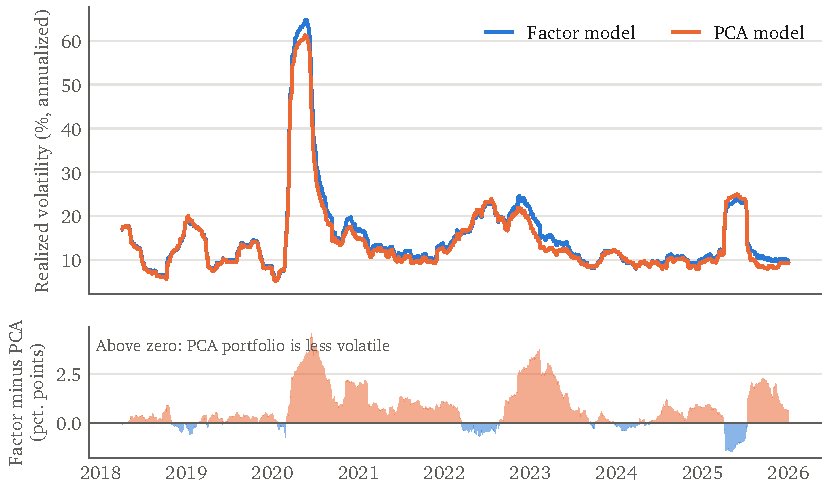
\includegraphics[width=\linewidth]{rolling_volatility.pdf}
\caption{Rolling three-month volatility of each model's minimum-variance portfolio (top)
and the difference between them (bottom). The two move together, and PCA is usually a little
lower.}
\label{fig:vol}
\end{figure}

\subsection{PCA tracked the index slightly more closely}

Tracking error was 1.74\% for PCA against 1.80\% for the factor model. The gap is significant
(interval 0.01 to 0.11 points) but small, at about six hundredths of a percentage point. In the three stress periods we examined separately, PCA
was ahead each time, by 0.31 points in the 2020 crash, 0.08 in the 2022 rate increases, and
0.02 in the March 2023 bank failures.

\subsection{The factor model traded less}

The factor model's minimum-variance portfolio turned over 0.208 of its value per rebalance
against 0.278 for PCA, about 25\% less. This advantage was specific to the minimum-variance
portfolio, because on the tracking portfolio the two models traded almost identically (0.081
and 0.082). The factor model's Sharpe ratio was also higher, 0.567 against 0.520, though we
did not test that difference for significance and I treat it as suggestive only.

\section{Why the two models differ}

Most of the differences between the two models can be traced to how each one spreads
variance across its risk drivers. Figure~\ref{fig:spectrum} shows how much of total variance
each model attributes to its largest drivers. Both agree on the single biggest driver, the
overall market, which accounts for about 43\%. Beyond that first driver the models diverge,
with PCA's top ten drivers explaining 64.6\% of variance and the factor model's explaining
53.7\%.

\begin{figure}[!htb]
\centering
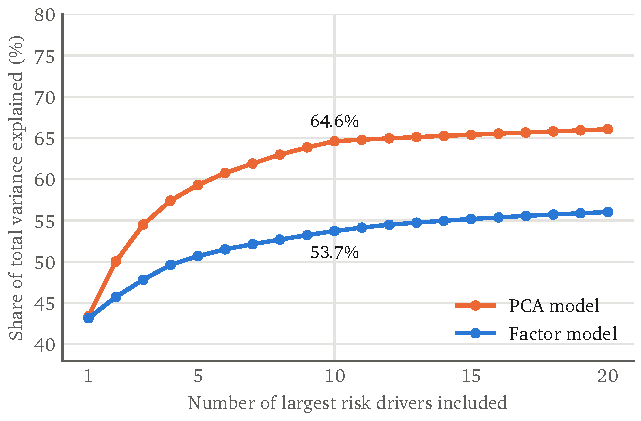
\includegraphics[width=0.78\linewidth]{variance_explained.pdf}
\caption{Cumulative share of variance explained by each model's largest risk drivers, on
the full universe. PCA concentrates risk into fewer, stronger drivers.}
\label{fig:spectrum}
\end{figure}

PCA's drivers are fitted directly to how these particular stocks moved, so with hundreds of
stocks and plenty of data it captures real structure that twenty pre-named factors miss.
That is its advantage on a broad portfolio. The same flexibility becomes a weakness when
there is less data to fit, because the smaller patterns it finds start to be noise. A factor
model cannot overfit in that way, since its structure is fixed in advance. This suggested a
prediction we could test: the factor model should do relatively better as the portfolio gets
smaller.

% =====================================================================
\section{Robustness checks}

Before accepting the result, we tested it against the objections we expected a skeptical
reader to raise.

\subsection{Giving both models the same amount of history}

The two models weighted history differently, and it was possible that this, not the choice
of factors, drove the result. We forced the factor model onto exactly the same two-year
window as PCA and also tried several faster weighting speeds. The results barely moved, with
volatility going from 17.93\% to 17.86\%, still significantly above PCA. The faster speeds
gained a little on volatility but gave back some of the turnover advantage, so the
difference in history windows does not explain the gap.

\subsection{How the winner changes with portfolio size}

To test the prediction from the previous section, we reran the entire comparison on
universes made up of the largest 15, 50, 100, 250, and 500 names in the index.
Figure~\ref{fig:crossover} shows a clean reversal, in which the factor model tracks better on
the small universes, PCA tracks better on the large ones, and the two are level at around
100 names.

\begin{figure}[!htb]
\centering
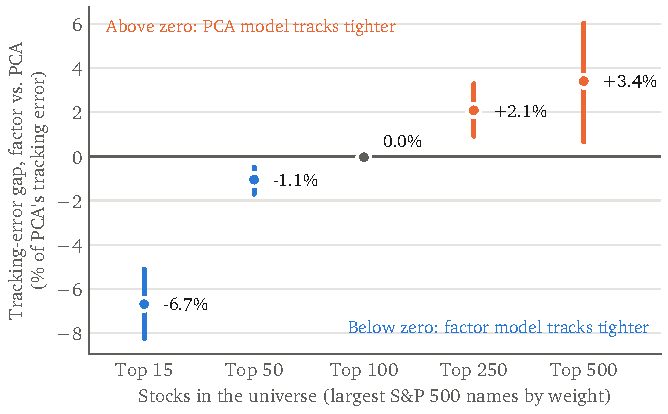
\includegraphics[width=0.78\linewidth]{universe_crossover.pdf}
\caption{Tracking-error gap between the models by universe size, as a percentage of PCA's
tracking error, with 95\% bootstrap intervals. Points are colored by the model that is
significantly better and gray where neither is.}
\label{fig:crossover}
\end{figure}

This test had a weakness, because choosing the largest 50 names changes two things at once.
The universe becomes smaller, and it also becomes made up entirely of very large companies.
To separate the two effects, we built 50-name and 100-name universes by random draw and by
sampling evenly across company sizes, eight times each. At 50 names the factor model's
advantage survived, winning on volatility in 75\% of random draws, while at 100 names it
mostly disappeared, with PCA winning 62\% of random draws. The reversal is therefore partly
a real small-universe effect and partly an effect of the very largest companies. The
evidence is fairly strong about where the reversal happens, but it does not establish why
it happens.

\subsection{Whether both models misjudge risk by the same amount}

Both models predicted less risk than actually occurred, by about 35\% on the
minimum-variance portfolio, mostly because of the 2020 crash. What matters for a comparison
is whether the error favors one side, and it did not, since the two models' ratios of
realized to predicted risk were 1.347 and 1.357. The shared error is a reason not to trust
either model's absolute forecast without correction, but it does not change which model is
ahead.

% =====================================================================
\section{Improving the factor model}

\subsection{Rebuilding the size factor}

The size score we started with was a percentile rank from 0 to 1. Because a rank flattens
out at the top, it could not distinguish the largest company in the index from the tenth largest,
and those companies dominate the S\&P 500. We rebuilt the factor from the logarithm of
market capitalization. Every headline number for the factor model improved slightly, and
the tracking-error gap to PCA narrowed from 0.059 to 0.050 points and was no longer
significant (interval $-0.01$ to $0.12$). The volatility gap remained.

\subsection{Blending the two models}

The simplest way to combine the models is a weighted average of their covariance matrices,
$\Sigma = \alpha\,\Sigma_{\text{factor}} + (1-\alpha)\,\Sigma_{\text{PCA}}$. An average of
two valid covariance matrices is always itself valid, so the blend required very little new
code:

\begin{lstlisting}
def make_blend_builder(alpha, factor_builder, pca_builder):
    """Covariance = alpha * factor + (1 - alpha) * PCA, on the tickers both models cover."""
    def build(as_of, tickers, ctx):
        f = factor_builder(as_of, tickers, ctx)
        p = pca_builder(as_of, list(f.index), ctx)
        common = [t for t in f.index if t in p.index]
        return alpha * f.loc[common, common] + (1.0 - alpha) * p.loc[common, common]
    return build
\end{lstlisting}

\begin{table}[H]
\centering\small
\begin{tabular}{@{}lrrr@{}}
\toprule
\textbf{Weight on factor model} & \textbf{Tracking error} & \textbf{Volatility} & \textbf{Turnover} \\
\midrule
0\% (pure PCA) & 1.744\% & 17.07\% & 0.278 \\
25\% & 1.736\% & 17.31\% & 0.278 \\
50\% & 1.739\% & 17.45\% & 0.269 \\
75\% & 1.751\% & 17.53\% & 0.250 \\
100\% (pure factor) & 1.803\% & 17.93\% & 0.208 \\
\bottomrule
\end{tabular}
\caption{Results across blend weights. Volatility and turnover are for the
minimum-variance portfolio.}
\label{tab:blend}
\end{table}

In Table~\ref{tab:blend} the 25\% blend has the lowest tracking error of all, lower than
either model alone, and in our first draft we reported that as the blend beating PCA. When
we later ran the bootstrap on it, Figure~\ref{fig:blend} showed that the blend's edge over
PCA was within the noise. The result that does hold up is that the blend is significantly
better than the factor model alone, so we corrected the claim to say that the blend matches
PCA on tracking but does not beat it.

\begin{figure}[!htb]
\centering
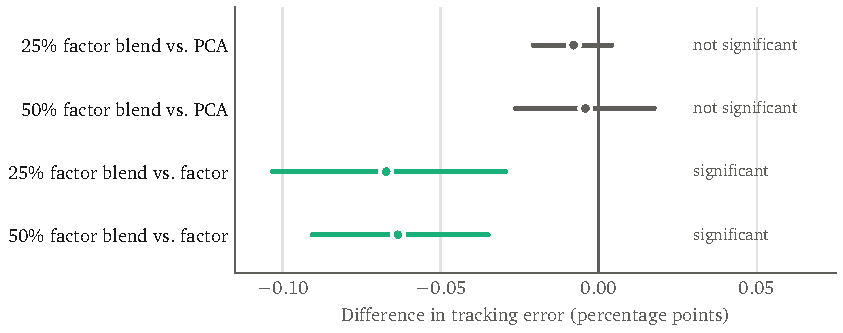
\includegraphics[width=0.84\linewidth]{blend_significance.pdf}
\caption{Tracking-error differences for the blended model, with 95\% bootstrap intervals.
Left of zero means the blend is better. An interval that crosses zero means the difference could be chance.}
\label{fig:blend}
\end{figure}

We also tried a more elaborate combination that modeled the factor model's leftover risk
with a second layer of statistical factors. This version performed worse, with volatility
rising to 18.26\% and no significant gain in tracking, so the simple average outperformed
the more complex approach.

\subsection{Accounting for trading costs}

Since the factor model trades less, we expected it to look better once trading costs were
included, and it did, though only modestly. At a cost of 25 basis points on turnover, the factor model's Sharpe
advantage on the minimum-variance portfolio widened from 0.047 to 0.061. Costs did not
change the ranking on volatility or tracking error at any level we tried.

% =====================================================================
\section{Application to tax-loss harvesting}

When a stock is sold to realize a loss, the portfolio needs a replacement that behaves as
much like it as possible, and the covariance matrix is what chooses that replacement. We
simulated 57,600 such swaps across the test period and compared the choices made by PCA, the
factor model, and two blends.

\begin{figure}[!htb]
\centering
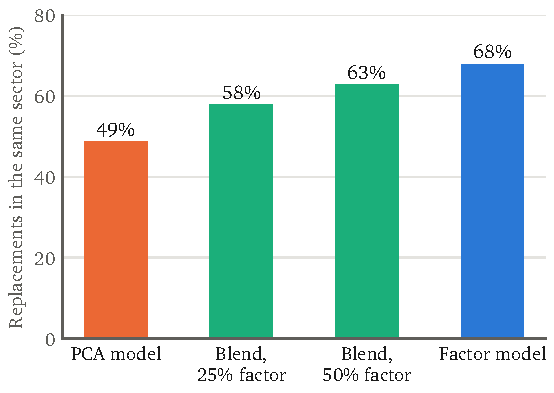
\includegraphics[width=0.62\linewidth]{tlh_sector_match.pdf}
\caption{How often each model's chosen replacement is in the same sector as the stock being
sold.}
\label{fig:tlh}
\end{figure}

\subsection{The factor model picked more recognizable replacements}

The factor model's choice was in the same sector as the stock being sold 68\% of the time,
against 49\% for PCA (Figure~\ref{fig:tlh}). The two models chose the same replacement in only 19\% of swaps.
For an advisor explaining a trade to a client, a replacement from the same sector is much
easier to justify.

\subsection{The cost of more intuitive replacements}

The pure factor model's more intuitive picks came with a small cost, because its
replacements added somewhat more realized tracking risk per swap than PCA's (24.1\% against
23.2\%, annualized, for the two-stock swap in isolation). The 25\% blend added the least of
the four (23.1\%) while still matching sectors 58\% of the time. These risk differences are
small and we did not bootstrap them, so I would place the most weight on the sector result.

\subsection{Lower turnover did not create more harvesting opportunities}

We expected that a model which trades less would leave more positions free to harvest,
since recently traded stocks are blocked by the wash-sale rule. In practice the share of the
portfolio available to harvest was 0.244 for the factor model and 0.245 for PCA. The factor
model trades smaller amounts but in about as many names, and it is the number of names that
triggers the restriction.

% =====================================================================
\section{The strengths of each model}

\begin{table}[H]
\centering\small
\begin{tabularx}{\linewidth}{@{}>{\raggedright\arraybackslash}X>{\raggedright\arraybackslash}X@{}}
\toprule
\textcolor{pca}{\textbf{PCA model}} & \textcolor{factor}{\textbf{Fundamental factor model}} \\
\midrule
Lower volatility and tracking error on broad portfolios, significant in both cases. &
About 25\% less trading on the minimum-variance portfolio. \\\addlinespace[5pt]
An edge that survived every check we made on the fairness of the test. &
Better results on small portfolios of around 50 names. \\\addlinespace[5pt]
The stronger choice when the only goal is minimizing risk on a broad index. &
Named, readable risk drivers, and more intuitive tax-loss replacements. \\
\bottomrule
\end{tabularx}
\end{table}

Neither model is better in every setting. On a broad S\&P 500 portfolio judged on risk
alone, the evidence favors PCA, while for a concentrated portfolio, or one where trading
cost and explainability carry weight, it favors the factor model or a blend. The blend looks like the
most promising direction for further research, because it keeps much of what is good about
each, but our evidence for it comes from one universe and a simplified optimizer.

\section{Limitations}

\begin{itemize}
\item \textbf{The ``fundamental'' factors were partly derived from prices.} This is the most
important caveat. The style scores we had were daily point-in-time scores, but they were not
built from company financials as reported at the time. Until the model is rebuilt on true
point-in-time fundamentals, it is not a fully independent source of information from PCA,
and the comparison could change.
\item \textbf{The optimizer was a simplified stand-in.} The rankings should carry over to a
production optimizer, but the absolute levels would not.
\item \textbf{The tracking portfolio's own risk forecasts were poor.} Both models predicted
tracking error several times lower than what occurred. We ranked on realized results only,
so the comparison holds, but those forecasts should not be used.
\item \textbf{The universe has survivorship bias.} It was drawn from current index members
and omits companies that were removed or delisted, which flatters the absolute numbers for
both models about equally.
\item \textbf{The study covers a single index over a single period.} Every result here comes
from the S\&P 500 between 2018 and 2025, and other indexes or market regimes could behave
differently.
\end{itemize}

\section{My role in the project and lessons learned}

Tommy Bobitz and I worked on this as a pair for the whole summer, under the guidance of the
Alphathena team. We built the data pipeline and the model together. For the experiments, I
wrote the engine that runs several models through the same rolling test, and I ran the
history-window, blending, and size-factor experiments and the tax-loss harvesting swap
study. Tommy ran the universe-size, trading-cost, and calibration experiments. I wrote the
internal paper this one is based on, and we presented the findings to the team together.

The work was in Python, mainly pandas, NumPy, and SciPy, with results stored as Parquet
files and every figure regenerated from saved results.

I took three lessons from the project. The first is that a result I did not want was still
a useful result. We set out to show that the factor model was better, it turned out not to
be, and the project was more valuable because we reported that plainly. The second is that
the most valuable hours were the ones spent questioning our own comparison. The blend looked
like a win until we tested it properly, and the size reversal looked simpler than it was
until we randomized the universes. The third is how much care it takes to keep a model from
seeing the future, since most of the ways a backtest can mislead are subtle and easy to
miss.

% =====================================================================
\clearpage
\appendix
\section{Appendix: the significance test}

This is the block bootstrap used throughout the paper. It resamples the daily results in runs of random
length, so each resample keeps the short-term persistence of the original series, and
recomputes the difference between the two models each time.

\begin{lstlisting}
def stationary_block_bootstrap(a, b, B=2000, mean_block=21, seed=42):
    """Bootstrap the realized difference in annualized volatility between two
    paired daily return series. Returns (point estimate, 2.5%, 97.5%, draws)."""
    rng = np.random.default_rng(seed)
    a, b = np.asarray(a), np.asarray(b)
    n, p = len(a), 1.0 / mean_block

    def stat(idx):
        return ann_vol(a[idx]) - ann_vol(b[idx])

    draws = np.empty(B)
    for k in range(B):
        idx, t = np.empty(n, dtype=int), 0
        while t < n:
            start = rng.integers(0, n)           # each block starts at a random day
            length = max(1, rng.geometric(p))    # and has a random length, mean 21
            for j in range(length):
                if t >= n:
                    break
                idx[t] = (start + j) % n         # wrap around the end of the sample
                t += 1
        draws[k] = stat(idx)
    lo, hi = np.percentile(draws, [2.5, 97.5])
    return stat(np.arange(n)), lo, hi, draws
\end{lstlisting}

\section{Appendix: terms}

\begin{description}[leftmargin=0pt,itemsep=0.3em]
\item[Covariance matrix.] A table of how much every pair of stocks tends to move together,
and the main input to a portfolio optimizer.
\item[Factor.] A shared driver of returns that affects many stocks at once, such as the
overall market, a sector, or a characteristic like company size.
\item[PCA.] Principal component analysis, a statistical method that finds the patterns
explaining the most variance in a set of returns, without naming them.
\item[Minimum-variance portfolio.] The portfolio with the lowest predicted risk, given a
covariance matrix. Ours was long-only with a cap on each position.
\item[Tracking error.] The volatility of the difference between a portfolio's returns and
its benchmark's.
\item[Turnover.] The fraction of a portfolio's value traded at a rebalance.
\item[Out of sample.] Scored on data that was not available when the model was built.
\item[Wash-sale rule.] A US tax rule that disallows a loss if the same security is bought
again within 30 days of the sale.
\end{description}

\end{document}
